%! Author = Len Washington III
%! Date = 1/15/24

% Preamble
\documentclass[lab=1,title={Speaking rate},turnin=false]{com310lab}

\newcommand{\wpm}{\mbox{Words per minute} = \frac{\mbox{\# words in speech sample}}{\mbox{duration of speech sample, in seconds}} \times 60 \mbox{ seconds}}
\newcommand{\sps}{\mbox{Syllables per second} = \frac{\mbox{\# syllables in speech sample}}{\mbox{duration of speech sample, in seconds}}}

% Document
\begin{document}

\maketitle

\begin{overview}
	Speaking rate refers to how fast or slow one speaks.
	For example, many people describe the variety of English from the rural American South as exhibiting a ``drawl'' that is characterized by slow speech, among other attributes.
	In contrast, speech from the urban North East is sometimes described as fast and under-articulated.
	In addition, the speech of women is often described as faster, compared to the speech of men.
	This claim about gender differences in speaking rate is seen not only in popular accounts of speech, but also in supposedly academic publications, e.g. Brizendine (2007), The Female Brain.
	(All of these claims, by the way, turn out to be false, but that’s another matter).
\end{overview}


\begin{problem}
	Various methods are used to measure speaking rate.
	One method estimates the number of words-per-minute of a speech sample, while another method estimates the number of syllables-per-second.
	They are calculated as follows:\\

	\begin{equation*}
	\begin{aligned}
		&\wpm\\
		&\sps
	\end{aligned}
	\end{equation*}\\

	In theory, both methods should yield similar results: speech found to be fast using one method should also be seen as fast using the other.
	Your job is to determine whether this expectation is true and explain why.
\end{problem}

\begin{task}
	Record the paragraph below using any voice recorder app.
	For example, ``voice memos'' on an iPhone will work, so long as you are able to find start and end times for any sentence.
	If you prefer, you can also use any of the recorded files in the ``Lab 1 files'' folder from past students who have agreed to let other students use their files.
	\begin{displayquote}
		Today was busy with preparations.
		Many of the students collected several important statements.
		John gave the book to Mark then put the keys on the chair.
		Sally opened the closet and removed a sweater.
		Fred closed the door and left the room.
		Mary delivered the computer to Susan then handed the papers to the teacher.
		All of the class had lots of things to do.
		Eventually, everyone completed the task they needed to perform.
	\end{displayquote}
	Then, compute the speaking rate for each sentence, using both words-per-minute (w.p.s.) and syllables-per-second (s.p.s) for each sentence as described above.
	You need no special tools to count the number of words and syllables in each sentence.
	If you need help with counting syllables, consult any dictionary--wiktionary is fine.
	To measure the duration of the speech sample, open the recording of your file, delete any pauses or false starts, and then select one sentence at a time and note its duration in seconds.
	Now, examine differences across certain sentences.
	For the purposes of this lab, ignore the first and last sentences.
	The other sentences are numbered as follows:
	\begin{displayquote}
		Sentence 1: Many of the students$\dots$\\
		Sentence 2: John gave$\dots$\\
		Sentence 3: Sally opened$\dots$\\
		Sentence 4: Fred closed$\dots$\\
		Sentence 5: Mary delivered$\dots$\\
		Sentence 6: All of$\dots$\\
	\end{displayquote}
	Compare w.p.m.\ and s.p.s.\ for the odd-numbered sentences to the same measures for the even-numbered sentences.
	Generate a table or graph showing your results.
	Summarize the results, and address the problem raised above, namely whether measures of speaking rates are consistent.
	If you find any differences, use the data to offer an explanation.
	(Hint: the measures are unlikely to be consistent with each other).
\end{task}

\begin{writeup}
	Follow the format for writing up phonetics lab reports and turn in your report on the day it is due.
\end{writeup}

\pagebreak

\labtitle

\begin{topic}
	This lab focuses on comparing different methods of measuring the rate that people talk at.
\end{topic}

\begin{issue}%TODO: Issue
	The topic revolving around the rate that we speak at has been debated on for years;
	with members from different regions commenting that the difference in speaking rates for the same language was very noticeable.
	To analyze this phenomenon, a number of sentences will be recorded and measured to see how certain rate measurements compare to each other.
\end{issue}

\begin{hypothesis}%TODO: Hypothesis
	The initial hypothesis is that there will be a consistent ratio between the measurement rates of words per minute and syllables per second.
	The basis of this hypothesis is that since people will normally speak at a consistent rate, the measurement rates will have similar changes as well.
\end{hypothesis}

\begin{method}%TODO: Review Method
	This lab was conducted by measuring the author speak the following sentences:
	\begin{table}[H]
	    \centering
		\caption{Sentences used for the Lab.}
		\label{tab:sentences}
		\begin{tabular}{|c|l|}
			\hline
			{\centering\textbf{Sentence ID}} & {\centering\textbf{Sentence}}\\
			\hline
			0 & ``Today was busy with preparations.''\\
			1 & ``Many of the students collected several important statements.''\\
			2 & ``John gave the book to Mark then put the keys on the chair.''\\
			3 & ``Sally opened the closet and removed a sweater.''\\
			4 & ``Fred closed the door and left the room.''\\
			5 & ``Mary delivered the computer to Susan then handed the papers to the teacher.''\\
			6 & ``All of the class had lots of things to do.''\\
			7 & ``Eventually, everyone completed the task they needed to perform.''\\
			\hline
		\end{tabular}
	\end{table}
	Each sentence was spoken and recorded by the author, and then analyzed using \href{https://www.fon.hum.uva.nl/praat/}{Praat}.
	The start and end times for each sentence were recorded, so the total amount of time for each sentence could be calculated.
	From there, the number of words and syllables for each sentence were found using Python and \href{https://rhymebrain.com/api.html}{RhymeBrain}.
	Using all of the information, the words per minute and syllables per second were calculated using the two following equations:
	\begin{equation}\wpm\label{eq:wpm}\end{equation}
	\begin{equation}\sps\label{eq:sps}\end{equation}
	The results taken from sentences 1--6 had their words per minute graphed against their syllables per second, and grouped depending on if their sentence id was odd or even.
\end{method}

\begin{results}%TODO: Results

	\makebox[1 \textwidth][c]{
		\newcolumntype{C}[1]{>{\centering\arraybackslash}p{#1\textwidth}}
			\begin{threeparttable}
				\rowcolors{1}{white}{SkyBlue1!50}
				\caption{Results from the Lab.}
				\label{tab:data}
				\begin{tabular}{|C{0.1}C{0.2}C{0.15}C{0.15}C{0.23}C{0.23}|}
	\hline
	Sentence Number&Sentence Duration (s)&Words per Sentence&Syllables per Sentence&Words per Minute (w.p.m)&Syllables per Seconds (s.p.s)\\
0&2.950393&5&10&101.6813692277605&3.3893789742586833\\
1&3.734091&8&16&128.54534075361315&4.284844691787105\\
2&3.826291&13&13&203.85276498833989&3.397546083138998\\
3&3.641891&8&13&131.79966121995412&3.5695741580404245\\
4&3.088693&8&8&155.40553884766146&2.590092314127691\\
5&5.393687&13&22&144.61350834781476&4.078842543143494\\
6&2.443294&10&10&245.5701196826907&4.092835328044845\\
7&3.964591&9&19&136.2057271481472&4.792423732990364\\
\hline\end{tabular}
%				\begin{tablenotes}
%					\small
%					\item
%				\end{tablenotes}
			\end{threeparttable}
	}

	\begin{figure}[H]
		\centering
		\caption{A scatter plot showing the words per minutes against the syllables per second of \hyperref[tab:data]{sentences} 1--6.}
		\label{fig:results}
		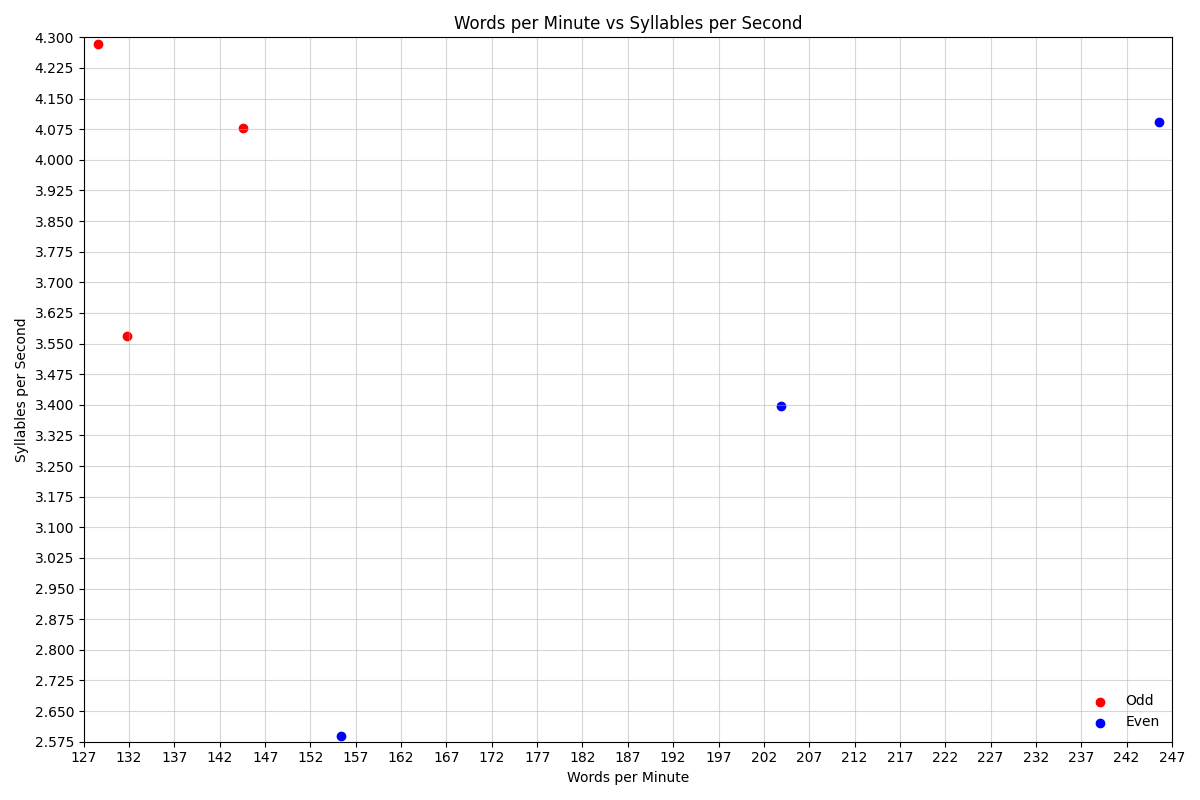
\includegraphics[width=\textwidth]{washington_lab1_graph}
	\end{figure}
\end{results}

% TODO: Discuss how the even sentences have the same number of syllables as words, whereas the odds don't. For the 1:1 syllable:word ratio sentences, the slope is seems about 1 (use washmath to find the actual slope), whereas the odd sentences vary due to the different rations for each sentence, however, there seems to be a 1:2 ratio of words:syllables, which would track if sentence 3 wasn't an outlier.
\begin{discussion}%TODO: Discussion
	The graphed results show that there is a relationship between the word per minute and syllables per second of each group.
	Each of the sentences in the ``even'' group had the same number of syllables and words in each sentence;
	and the results state that there is a 100\% correlation between the two groups.\\

	There was no strong correlation recorded within the ``odd'' group, however, if the data point for Sentence 3 were removed, then a stronger relationship could be found for the ``odd'' group.
	On average, each sentence in the ``odd'' group had 1.5 syllables per word, and without Sentence 3, the average ratio is about 1.2, much closer to the measured average.
\end{discussion}

\end{document}